\documentclass[10pt]{beamer}

\usepackage[english]{babel}
\usepackage[utf8]{inputenc}
\usepackage{amsmath,amssymb,amsthm,latexsym}
\usepackage{mathrsfs}
\usepackage[all]{xypic}
\usepackage{tikz}
\usetikzlibrary{arrows,shapes,automata}

\newcommand{\cat}[1]{\mathscr{#1}}
\newcommand{\lcat}[1]{\mathbf{#1}}
\newcommand{\C}{\cat{C}}
\newcommand{\D}{\cat{D}}
\renewcommand{\L}{\cat{L}}
\newcommand{\comp}{\circ}
\newcommand{\size}[1]{\lVert#1\rVert}
\newcommand{\sizein}[1]{\size{#1}^\mathrm{in}}
\newcommand{\sizeout}[1]{\size{#1}_\mathrm{out}}
\DeclareMathOperator{\ob}{ob}
\DeclareMathOperator{\Hom}{Hom}
\DeclareMathOperator{\id}{id}
\DeclareMathOperator{\Id}{Id}
\newcommand{\N}{\mathbb{N}}
\newcommand{\Z}{\mathbb{Z}}
\newcommand{\Complex}{\mathbb{C}}
\newcommand{\R}{\mathbb{R}}
\newcommand{\K}{\mathbb{K}}
\newcommand{\LK}{\mathbb{L}}
\newcommand{\ra}{\rightarrow}
\newcommand{\la}{\leftarrow}
\DeclareMathOperator{\Time}{t}
\DeclareMathOperator{\Space}{s}
\DeclareMathOperator{\coTime}{co-t}
\DeclareMathOperator{\coSpace}{co-s}
\DeclareMathOperator{\Par}{Par}
\DeclareMathOperator{\Tr}{Tr}
\DeclareMathOperator{\rev}{rev}
\newcommand{\computes}{\vdash}
\renewcommand{\u}{\underline}
\renewcommand{\o}{\overline}


\mode<presentation>{%
  \usetheme[]{Madrid}
  \usecolortheme{seahorse}
  \usecolortheme{rose}
  \usefonttheme[onlymath]{serif}
}


\title{On the transposition of black box matrices}
\author[L. De Feo]{L.~De~Feo\\{\footnotesize(joint work in progress with É.~Schost)}}
\institute[TANC, LIX]{Projet TANC, LIX, École Polytechnique}
\date[Typical, February 11, 2010]{Séminaire TypiCal\\February 11, 2010}

\AtBeginSection[]
{
  \begin{frame}<beamer>
    \frametitle{Plan}
    \tableofcontents[currentsection]
  \end{frame}
}


\begin{document}

\begin{frame}
  \titlepage
\end{frame}

\section{Black-box model}

\begin{frame}
  \frametitle{The power iteration}

  \begin{block}{Find the largest eigenvalue}
    \begin{center}
      $A$ a real-valued matrix, $b_0$ a random vector

      \[b_{i+1} = \frac{A^i \cdot b_i}{c_i}\]
      
      $b_i$ (slowly) converges to the largest eigenvalue.
    \end{center}
  \end{block}

  \begin{itemize}
  \item Numerical analysis (inexact algorithm),
  \item unbounded number of iterations,
  \item \alert{suitable for sparse matrices},
  \item \alert{does not use the block structure of $A$, only evaluates
      $A\cdot b$}.
  \item Used by Google page ranking algorithm \cite{google}.
  \end{itemize}
\end{frame}

%%

\begin{frame}
  \frametitle{From numerical algorithms to exact algorithms}

  \begin{block}{Solving \alert{sparse} linear equations over finite
      fields \cite{Wie86}}
    \begin{itemize}
    \item \alert{Exact} algorithm, \alert{bounded} number of iterations,
    \item Only evaluates products $A\cdot b$, suitable for sparse
      matrices.
    \item Contains exact algorithms for sparse determinant, minimal
      polynomial and inverse (of course).
    \end{itemize}
  \end{block}
\end{frame}

%%

\begin{frame}
  \frametitle{From sparse to black-box matrices}

  \begin{block}{Symbolic calculus}
    \begin{itemize}
    \item Compute with \alert{symbolic} objects,
    \item Matrices with coefficients in a ring $R$ represented as
      \emph{computer programs}.
    \item \emph{Black-box model} of complexity.
    \end{itemize}
  \end{block}

  \[\xymatrix{
    b\ar[r]  & \rule{10ex}{2em} \ar[r] & A\cdot b
  }\]

  \begin{block}{Not only sparse matrices!}
    \[\begin{pmatrix}
      1 & a_1 & a_1^2 & \cdots & a_1^{n-1}\\
      &&\vdots \\
      1 & a_m & a_m^2 & \cdots & a_m^{n-1}\\
    \end{pmatrix}\]
    \begin{itemize}
    \item \cite{KaTr90} extends to black-box polynomials (GCD,
      Factorizations, \dots)
    \end{itemize}
  \end{block}
\end{frame}

%%
%%

\section{Algebraic complexity}

\begin{frame}
  \frametitle{Measuring the complexity of black-box algorithms}

  \begin{block}{Complexity of a black-box algorithm}
    \begin{itemize}
    \item Count number of black-box calls (number of matrix-vector products)
    \item plus number of \emph{offline} operations in $R$
    \end{itemize}

    \textbf{Question:} (\cite{Ka2k}) Is it possible to solve any
    linear algebra operation in
    \begin{itemize}
    \item $O(n)$ black-box calls,
    \item $n^2(\log n)^{O(1)}$ offline operations,
    \item $O(n)$ storage (not counting black-box storage)?
    \end{itemize}

    \begin{center}
      \alert{This question is open i.e. for characteristic polynomials!}
    \end{center}
  \end{block}

  \begin{block}{Complexity of the black-box}
    \begin{itemize}
    \item Count the number of $+, \times$ operations in $R$,
    \item count the number of elements of $R$ to be stored.
    \end{itemize}
  \end{block}
\end{frame}

%%

\begin{frame}
  \frametitle{Arithmetic circuits}

  \begin{block}{Algebraic complexity}
    \centering Fix a (commutative) ring $R$. We construct circuits that
    evaluate arithmetic functions.
  \end{block}


  \begin{center}
    Three gates: Addition, duplication, multiplication by a fixed
    element $a\in R$.
    
    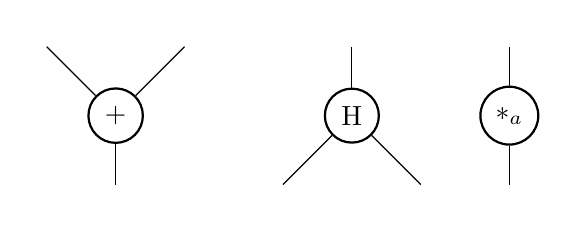
\begin{tikzpicture}
      \tikzstyle{node}=[circle,thick,draw=black,minimum size=4mm]
      
      \begin{scope}
        \node(in1){};
        \node(nop1)[right of=in1]{};
        \node(in2)[right of=nop1]{};
        \node(nop2)[right of=in2]{};
        \node(in3)[right of=nop2]{};
        \node(nop3)[right of=in3]{};
        \node(in4)[right of=nop3]{};
        
        \node[node](plus)[below of=nop1]{$+$}
        edge(in1)
        edge(in2);
        \node(nop)[below of=nop2]{};
        \node[node](hub)[below of=in3]{H}
        edge(in3);
        \node[node](times)[below of=in4]{$*_a$}
        edge(in4);
        
        \node(out1)[below of=plus]{}
        edge(plus);
        \node(nop5)[right of=out1]{};
        \node(out2)[below of=nop]{}
        edge(hub);
        \node(nop6)[below of=hub]{};
        \node(out3)[right of=nop6]{}
        edge(hub);
        \node(out4)[below of=times]{}
        edge(times);
      \end{scope}
    \end{tikzpicture}
  \end{center}
\end{frame}

%%

\begin{frame}
  \frametitle{Arithmetic circuits}

  \begin{columns}
    \begin{column}{0.6\textwidth}
      \centering
      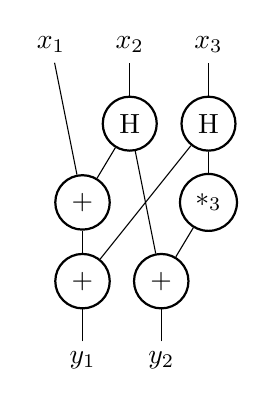
\begin{tikzpicture}
        \tikzstyle{node}=[circle,thick,draw=black,minimum size=4mm]
        
        \begin{scope}
          \node(x1){$x_1$};
          \node(x2)[right of=x1]{$x_2$};
          \node(x3)[right of=x2]{$x_3$};
          
          \node[node](d1)[below of=x2]{H}
          edge(x2);
          \node[node](d2)[below of=x3]{H}
          edge(x3);
          
          \node[node](p1)[below of=d1,xshift=-6mm]{$+$}
          edge(x1)
          edge(d1);
          \node[node](m1)[below of=d2]{$*_3$}
          edge(d2);
          
          \node[node](p2)[below of=p1]{$+$}
          edge(p1)
          edge(d2);
          \node[node](p3)[right of=p2]{$+$}
          edge(d1)
          edge(m1);
          
          \node(y1)[below of=p2]{$y_1$}
          edge(p2);
          \node(y2)[below of=p3]{$y_2$}
          edge(p3);
        \end{scope}
      \end{tikzpicture}
    \end{column}
    \begin{column}{0.4\textwidth}
      \begin{align*}
        y_1 &= x_1 + x_2 + x_3\\
        y_2 &= x_2 + 3x_3
      \end{align*}
      
      \Large
      \begin{gather*}
        \begin{pmatrix}
          1 & 1 & 1\\
          0 & 1 & 3
        \end{pmatrix}
      \end{gather*}
    \end{column}
  \end{columns}
  
  \smallskip
  
  \begin{center}
    \Large
    Complexity = number of gates
  \end{center}
\end{frame}

%%

\begin{frame}
  \frametitle{Arithmetic Circuits: uniform vs. non-uniform}

  \begin{definition}[Algorithm]
    An algorithm $A$ is a family of arithmetic circuits indexed by a
    size function $s_A:\N\rightarrow\mathcal{C}_R$. The output of $A$
    on input $x\in R^\ast$ is the output of $s_A(|x|)$ on input $x$.
  \end{definition}

  \begin{definition}[Uniform algorithm]
    An algorithm is said to be \emph{uniform} if there is a $\log
    n$-space bounded touring machine which on input $1^n$ outputs
    $s(n)$.
  \end{definition}

  \begin{itemize}
  \item We will extend the definition to allow the size function to be
    a function $s:\mathcal{P}\rightarrow\mathcal{C}_R$ for an
    arbitrary countable set $\mathcal{P}$. We call $\mathcal{P}$ the
    \emph{parameter space}.
  \item \alert{Any Touring-undecidable problem has a trivial
      \emph{polynomial-size} algorithm deciding it.}
  \end{itemize}
\end{frame}

%%
%%

\section{The transposition theorem}

\begin{frame}
  \frametitle{Transposition of an arithmetic circuit}

  \begin{columns}
    \begin{column}{0.6\textwidth}
      \centering
      \begin{tikzpicture}
        \tikzstyle{node}=[circle,thick,draw=black,minimum size=4mm]
        
        \begin{scope}
          \node(x1){$x_1$};
          \node(x2)[right of=x1]{$x_2$};
          \node(x3)[right of=x2]{$x_3$};
          
          \node[node](d1)[below of=x2]{H}
          edge(x2);
          \node[node](d2)[below of=x3]{H}
          edge(x3);
            
          \node[node](p1)[below of=d1,xshift=-6mm]{$+$}
          edge(x1)
          edge(d1);
          \node[node](m1)[below of=d2]{$*_3$}
          edge(d2);
          
          \node[node](p2)[below of=p1]{$+$}
          edge(p1)
          edge(d2);
          \node[node](p3)[right of=p2]{$+$}
          edge(d1)
          edge(m1);
          
          \node(y1)[below of=p2]{$y_1$}
          edge(p2);
          \node(y2)[below of=p3]{$y_2$}
          edge(p3);
        \end{scope}
        
        \begin{scope}[xshift=3.2cm, yshift=-0.23\textheight]
          \node(x){\Huge $\leftrightarrow$};
        \end{scope}
        
        \begin{scope}[xshift=4cm, yshift=-0.425\textheight]
          \node(x1){$x_1'$};
          \node(x2)[right of=x1]{$x_2'$};
          \node(x3)[right of=x2]{$x_3'$};
          
          \node[node](d1)[above of=x2]{\alt<2>{$+$}{H}}
          edge(x2);
          \node[node](d2)[above of=x3]{\alt<2>{$+$}{H}}
          edge(x3);
          
          \node[node](p1)[above of=d1,xshift=-5mm]{\alt<2>{H}{$+$}}
          edge(x1)
          edge(d1);
          \node[node](m1)[above of=d2]{$*_3$}
          edge(d2);
          
          \node[node](p2)[above of=p1]{\alt<2>{H}{$+$}}
          edge(p1)
          edge(d2);
          \node[node](p3)[right of=p2]{\alt<2>{H}{$+$}}
          edge(d1)
          edge(m1);
          
          \node(y1)[above of=p2]{$y_1'$}
          edge(p2);
          \node(y2)[above of=p3]{$y_2'$}
          edge(p3);
        \end{scope}
      \end{tikzpicture}
    \end{column}
    \begin{column}{0.4\textwidth}
      \begin{align*}
        y_1 &= x_1 + x_2 + x_3\\
        y_2 &= x_2 + 3x_3
      \end{align*}
      
      \Large
      \begin{gather*}
        \begin{pmatrix}
          1 & 1 & 1\\
          0 & 1 & 3
        \end{pmatrix}\\
        \updownarrow\\
        \begin{pmatrix}
          1 & 0\\
          1 & 1\\
          1 & 3\\
        \end{pmatrix}
      \end{gather*}
    \end{column}
  \end{columns}
\end{frame}

%%

\begin{frame}
  \frametitle{History of the transposition theorem}

  \begin{block}{History}
    \begin{itemize}
    \item Originally discovered by \alert{Tellegen (1950)},
      \alert{Bordewijk (1956)} for \emph{electrical network theory}
      and by \alert{Kalman (1960)} for \emph{control theory};
    \item Graph-theoretic approach by \alert{Fettweis (1971)} for
      \emph{digital filters};
    \item \alert{Fiduccia (1972)}: transposition of \emph{bilinear
      algorithms};
    \item Special case of reverse mode in \emph{automatic differentiation}:
      \alert{Baur \& Strassen (1983)};
    \item In \emph{computer algebra}, popularized by \alert{Shoup},
      \alert{von zur Gathen}, \alert{Kaltofen},\dots
    \item \alert{\cite{BLS03}} improve algorithms for
      polynomial evaluation.
    \end{itemize}
  \end{block}
  
  \begin{block}{Motivations}
    \begin{itemize}
    \item Existence result in \emph{complexity theory};
    \item \emph{Code transformation} technique;
    \item Improve $M^T \Leftrightarrow$ Improve $M$;
    \item {\bf Divides by $2$ the number of algorithms yet to be discovered.}
    \end{itemize}
  \end{block}
\end{frame}

%%

\begin{frame}[fragile]
  \frametitle{From non-uniform to uniform circuits?}
  
  {\large
    \begin{itemize}
    \item The transposition theorem applies to non-uniform circuits.
    \item Is the transposed of an uniform circuit still uniform?
    \item What about complexity?
    \end{itemize}}

    \begin{columns}

    \begin{column}{0.5\textwidth}
      \begin{center}
        \begin{minipage}{0.7\textwidth}
\begin{semiverbatim}
  for i = 1 to n-2 do
    a[i+1] = a[i] + a[i+1]
    a[i] = 0
  end for
\end{semiverbatim}
        \end{minipage}
      \end{center}
    \end{column}

    \begin{column}{0.5\textwidth}

      \begin{equation*}
        \begin{pmatrix}
          0 & \hdotsfor{3} & 0\\
          \vdots  &  &\vdots&& \vdots \\
          0 & \hdotsfor{3} & 0\\
          1 & \hdotsfor{3} & 1
        \end{pmatrix}
      \end{equation*}

    \end{column}
  \end{columns}


\end{frame}

%%

\begin{frame}[fragile]
  \frametitle{From non-uniform to uniform circuits?}

  \begin{columns}
    \begin{column}{0.5\textwidth}
      \begin{center}
        \begin{minipage}{0.7\textwidth}
\begin{semiverbatim}
  a[1] = a[0] + a[1]
  a[0] = 0
  a[2] = a[1] + a[2]
  a[1] = 0
  ...
  a[n-1] = a[n-2] + a[n-1]
  a[n-2] = 0
\end{semiverbatim}
        \end{minipage}
      \end{center}
    \end{column}

    \begin{column}{0.5\textwidth}
      \begin{center}
        \begin{minipage}{0.7\textwidth}
\begin{semiverbatim}
  a[n-2] = 0
  a[n-2] = a[n-2] + a[n-1]
  ...
  a[1] = 0
  a[1] = a[1] + a[2]
  a[0] = 0
  a[0] = a[0] + a[1]
\end{semiverbatim}
        \end{minipage}
      \end{center}
    \end{column}
    \end{columns}
  
  \vfill

  \begin{columns}

    \begin{column}{0.5\textwidth}
      \begin{center}
        \begin{minipage}{0.7\textwidth}
\begin{semiverbatim}
  for i = n-2 to 0 do
    a[i] = 0
    a[i] = a[i] + a[i+1]
  end for
\end{semiverbatim}
        \end{minipage}
      \end{center}
    \end{column}

    \begin{column}{0.5\textwidth}

      \begin{equation*}
        \begin{pmatrix}
          0 & \hdotsfor{3} & 0\\
          \vdots  &  &\vdots&& \vdots \\
          0 & \hdotsfor{3} & 0\\
          1 & \hdotsfor{3} & 1
        \end{pmatrix}
      \end{equation*}

    \end{column}
  \end{columns}
\end{frame}

%%

\begin{frame}[fragile]
  \frametitle{The case of multiplication}

  
  \begin{block}{The bilinearity of multiplication}
    \begin{columns}
      \begin{column}{0.3\textwidth}
        \begin{center}
          \begin{minipage}{0.7\textwidth}
            \footnotesize
\begin{verbatim}
Mult(x, y) {
  return x * y;
}
\end{verbatim}    
          \end{minipage}
        \end{center}
      \end{column}
      \begin{column}{0.7\textwidth}
        \begin{itemize}
        \item Multiplication \alert{is not linear},
        \item But \emph{Transposed multiplication} (aka \emph{Middle
          product}) is a very important operation: \cite{BLS03}, \cite{Sho95}
        \item fix \verb|x|, then $\verb|Mult|_{\verb|x|}$ \alert{is linear}.
        \end{itemize}
      \end{column}
    \end{columns}    
  \end{block}

  \begin{block}{Put $x$ in the parameter space}
    \begin{align*}
      s:R&\rightarrow\mathcal{C}_R\\
      x&\mapsto C_x
    \end{align*}
    Where $C_x$ is the circuit such that $C_x(y) = xy$.
  \end{block}

  \begin{center}
    \textbf{How do we automatically find it ?}
  \end{center}
\end{frame}

%%

\begin{frame}[fragile]
  \frametitle{The parameter space: \texttt{linear} and \texttt{const}
    variables}

  \begin{columns}
    \begin{column}{0.5\textwidth}
      \begin{center}
\begin{semiverbatim}
  Mult(const x, linear y) \{
    return x*y;
  \}
\end{semiverbatim}
      \end{center}
    \end{column}
    \begin{column}{0.5\textwidth}
      For notational convenience we write
      \[(\o{result})Mult(\u{x}, \o{y})\]
    \end{column}
  \end{columns}


  \begin{block}{Linear programs}
    A computer program  $P$
    \[(\o{A}, \ldots, \u{a}, \ldots)P(\o{Z}, \ldots, \u{z}, \ldots)\]
    is said to be \emph{linear} if for any $z,\ldots\in\mathcal{P}$
    and $Z_1,Z_2,\ldots\in R^\ast$
    \begin{align*}
      &(A_1, \ldots, a, \ldots)P(Z_1, \ldots, z, \ldots)\\
      &(A_2, \ldots, a, \ldots)P(Z_2, \ldots, z, \ldots)
    \end{align*}
    and if this implies
    \[(A_1 + A_2, \ldots, a, \ldots)P(Z_1 + Z_2, \ldots, z, \ldots)\]
  \end{block}
\end{frame}

%%
%%

\section{A transposable language}

\begin{frame}[fragile]
  \frametitle{TransAL: the Transposable Algebraic Language}

  \begin{block}{Algebraic types}
    \begin{itemize}
    \item \textbf{Prototypes}: {\tt Ring}, {\tt Module}, (optionally
      {\tt Algebra}, \dots)
    \item Declaring an algebraic type:
\begin{semiverbatim}
  type Ring R
  type Module M
\end{semiverbatim}
    \end{itemize}
  \end{block}

  \begin{block}{Declaring a function}
\begin{semiverbatim}
  fun (linear M A, const m)f(linear M Z, const M z, const n):
\end{semiverbatim}
  \end{block}

  \begin{block}{Other constructs}
    \begin{itemize}
    \item Standard types ({\tt int}, {\tt bool}, \ldots)
    \item {\tt if}, {\tt match}, recursion, {\tt let} binding,
    \item Algebraic operators $+$, $\times$, access to coordinate \verb|a[n]|,
    \item (Optionally) curryfication.
    \end{itemize}
  \end{block}
\end{frame}

%%

\begin{frame}[fragile]
  \frametitle{Automatic transposition: the general algorithm}

\begin{semiverbatim}
  fun (linear R res)scalar(linear M a, const n):
    if n = 0:
      res = 0
    else:
      res = a[n] + scalar(a, n-1)
\end{semiverbatim}

  \begin{block}{The algortithm}
    \begin{itemize}
    \item First run the algorithm in the normal direction to compute
      all the {\tt const} values,
    \item then run the algorithm backwards transposing each instruction.
    \end{itemize}
  \end{block}

\begin{semiverbatim}
  fun (linear M a)scalar^T(linear R res, const n):
    if n = 0:
      nop
    else:
      a[n] = res
      a += scalar^T(res, n-1)
\end{semiverbatim}
\end{frame}

%%

\begin{frame}
  \frametitle{Non-linear prediction and tail recursion}

  \begin{itemize}
  \item Permuting the order of the instructions may break tail/head
    recursion,
  \item this implies loss of efficiency,
  \item equivalently, in {\tt for} loops we have to precompute all the
    {\tt const} values of the loop,
  \item \alert{this seems to increase the space requirements of the
      algorithm}, but does not affect the number of arithmetic operations.
  \end{itemize}
\end{frame}

%%
%%

\section{Constness inference system}

\begin{frame}
  \frametitle{Automatic deduction of constness, a simple idea}

\end{frame}

%%

\begin{frame}
  \frametitle{The problem, relationship with generically quantified types}

\end{frame}

%%

\begin{frame}
  \frametitle{A simple algorithm}

\end{frame}

%%
%%

\section{Transalpyne}

\begin{frame}
  \frametitle{A Python implementation of TransAL}

  \begin{center}
    \Large
    \url{http://transalpyne.gforge.inria.fr/}
  \end{center}

  \begin{itemize}
  \item Compiler/interpreter written in python,
  \item python-like syntax,
  \item automated constness inference,
  \item smart handling of array sizes,
  \item will compile to other languages (Haskell? OCaml?).
  \end{itemize}
\end{frame}

%%
%%

\section{A categorical point of view}

\begin{frame}
  \frametitle{Arrows, not circuits !}

  \begin{columns}
    \begin{column}{0.3\textwidth}
      Covariant functor $F:\C\ra\D$
    \end{column}

    \begin{column}{0.25\textwidth}
      \begin{equation*}
        \xymatrix{
          A \ar[r]^f \ar[dr]_{h} & B \ar[d]^g \\
          & C
        }
      \end{equation*}
    \end{column}
    \begin{column}{0.05\textwidth}
      $\mapsto$
    \end{column}
    \begin{column}{0.35\textwidth}
      \begin{equation*}
        \xymatrix{
          F(A) \ar[r]^{F(f)} \ar[dr]_{F(h)} & F(B) \ar[d]^{F(g)} \\
          & F(C)
        }    
      \end{equation*}
    \end{column}
  \end{columns}

  \begin{columns}
    \begin{column}{0.3\textwidth}
      Contravariant functor $F:\C\ra\D$
    \end{column}

    \begin{column}{0.25\textwidth}
      \begin{equation*}
        \xymatrix{
          A \ar[r]^f \ar[dr]_{h} & B \ar[d]^g \\
          & C
        }
      \end{equation*}
    \end{column}
    \begin{column}{0.05\textwidth}
      $\mapsto$
    \end{column}
    \begin{column}{0.35\textwidth}
      \begin{equation*}
        \xymatrix{
          F(A) & F(B) \ar[l]_{F(f)} \\
          & F(C) \ar[u]_{F(g)} \ar[ul]^{F(h)}
        }    
      \end{equation*}
    \end{column}
  \end{columns}

  \begin{block}{Equivalence, duality}
    \begin{itemize}
    \item Equivalence if $F:\C\ra\D$ and $G:\D\ra\C$ covariant
    \item Duality if $F:\C\ra\D$ and $G:\D\ra\C$ contravariant 
    \end{itemize}
    and $\quad F\comp G \simeq \Id_\D\quad$ and $\quad G\comp F \simeq \Id_\C$.
  \end{block}
\end{frame}

%%

\begin{frame}
  \frametitle{Transposition as a contravariant functor}

\end{frame}

%%

\begin{frame}
  \frametitle{Some trivial applications}

\end{frame}

%%

\begin{frame}
  \frametitle{Some interesting problems}

  \begin{itemize}
  \item What's the relationship to the \emph{Categorical Abstract Machine}?
  \item Do these techniques generalise to other functors?
  \item Is it possible to design a generic framework in which a
    programmer could implement its own functor?
  \item Is it possible to gain on the space requirements?
  \item Optimise some of the algorithms?
  \end{itemize}
\end{frame}

%%
%%

\begin{frame}
  \frametitle{Bibliography}

  \begin{thebibliography}{1}
  
  \bibitem[B\"urgisser, Clausen, Shokrollahi]{BCS}P.~Bürgisser, M.~Clausen \& M.~A.~Shokrollahi,
    \newblock \emph{Algebraic Complexity Theory}.
    \newblock Springer, 1997.
    
  \bibitem[Bostan, Lercerf, Schost '03]{BLS03}A.~Bostan, G.~Lecerf \& E.~Schost,
    \newblock Tellegen's Principle into Practice.
    \newblock \emph{Proceedings of ISAAC 2003}.

  \bibitem[D.F., Schost '09]{DFS09}
    L.~De~Feo and {\'E}.~Schost.
    \newblock Fast arithmetics in Artin-Schreier towers over finite fields. 
    \newblock In \emph{ISSAC'09}, pages 127--134. ACM, 2010.

  \bibitem[Kaltofen '00]{Ka2k}
    E.~Kaltofen.
    \newblock Challenges of symbolic computation: my
    favorite open problems.
    \newblock \emph{Journal of Symbolic Computation}, 29(6):891--919, 2000.

  \bibitem[Kaltofen, Trager '90]{KaTr90}
    E.~Kaltofen, B.~M.~Trager.
    \newblock Computing with polynomials given by black boxes for their
    evaluations: greatest common divisors, factorization, separation of 
    numerators and denominators.
    \newblock \emph{J. Symb. Comput.}, 9:301--320, 1990.

  \end{thebibliography}
\end{frame}

\begin{frame}
  \frametitle{Bibliography}

  \begin{thebibliography}{1}
  
  \bibitem[Page, Brin, Motwani, Winograd '99]{google}
    L.~Page, S.~Brin, R.~Motwani and T.~Winograd.
    \newblock The PageRank Citation Ranking: Bringing Order to the Web.
    \newblock \emph{Technical Report}, Stanford InfoLab, 1999,
    \url{http://ilpubs.stanford.edu:8090/422/}.

  \bibitem[Papadimitriou]{Papa}
    C.~H.~Papadimitriou.
    \newblock \emph{Computational complexity}.
    \newblock Pearson Education, 1995.
    
  \bibitem[Pascal, Schost '06]{PS06}
    C.~Pascal and \'E.~Schost.
    \newblock Change of order for bivariate triangular sets.
    \newblock In \emph{ISSAC'06}, pages 277--284. ACM, 2006.
    
  \bibitem[Shoup '95]{Sho95}
    V.~Shoup.
    \newblock A new polynomial factorization algorithm and its implementation.
    \newblock \emph{J. Symb. Comp.}, 20(4):363--397, 1995.
    
  \bibitem[Wiedemann '86]{Wie86}
    D.~H.~Wiedemann.
    \newblock Solving Sparse Linear Equations Over Finite Fields.
    \newblock \emph{IEEE Trans. Inf. Theory}, vol. IT-32:54--62, 1986.

  \end{thebibliography}
\end{frame}

\end{document}





%%% Local Variables: 
%%% mode:flyspell
%%% ispell-local-dictionary:"british"
%%% mode: TeX-PDF
%%% TeX-master: t
%%% End: 
%
% LocalWords:  Tellegen